\documentclass[12pt]{amsart}
\usepackage[margin=1in]{geometry}
\usepackage{pbox}
\usepackage{graphicx}
\usepackage{booktabs} % Top and bottom rules for table
\usepackage{amsfonts, amsmath, amsthm, amssymb}
\usepackage{longtable,array,color,xcolor}
\usepackage[colorlinks = true,
            urlcolor  = blue]{hyperref}

\newcommand\narrowstyle{\SetTracking{encoding=*}{-50}\lsstyle}

\pagestyle{empty}

\usepackage[top=.6in,bottom=0.5in,left=0.5in,right=0.5in]{geometry}

\setlength{\parindent}{0pt}

\begin{document}
{\bf Math 320 -- Computer Methods in the Mathematical Sciences I.} Fall 2016.
\\[3mm]
\subsection*{MATLAB}
See the information here on how to access MATLAB through the university:
https://www.seas.upenn.edu/cets/software/matlab/

\subsection*{Coding Advice}
If you have not had much experience programming, don't panic!
Here are a few helpful tips:
\begin{enumerate}
\item {\bf Google is your friend.} Search for things like ``examples
MATLAB plot data'' and ``MATLAB ValueError''. If you are having
difficulty, someone else has before you.
\item {\bf Your friends are your friends.} Talk to people you
know who have worked in MATLAB or other programming languages, 
or talk to your classmates.
\item {\bf Discussion Section of Canvas.} The canvas site will
have discussion threads for each homework -- please ask and answer
questions there. 
\item {\bf Office hours!} Come to office hours with any questions!
Office hours will be held after class on Wednesday in 
DRLB 3N8D. (This is subject to change.)
\item {\bf Online tutorials.} If you want to get some hands-on
experience in MATLAB or Octave, look for an online tutorial. 
For example, the MATLAB Onramp is available through Mathworks.
\end{enumerate}

\begin{figure}[b!]
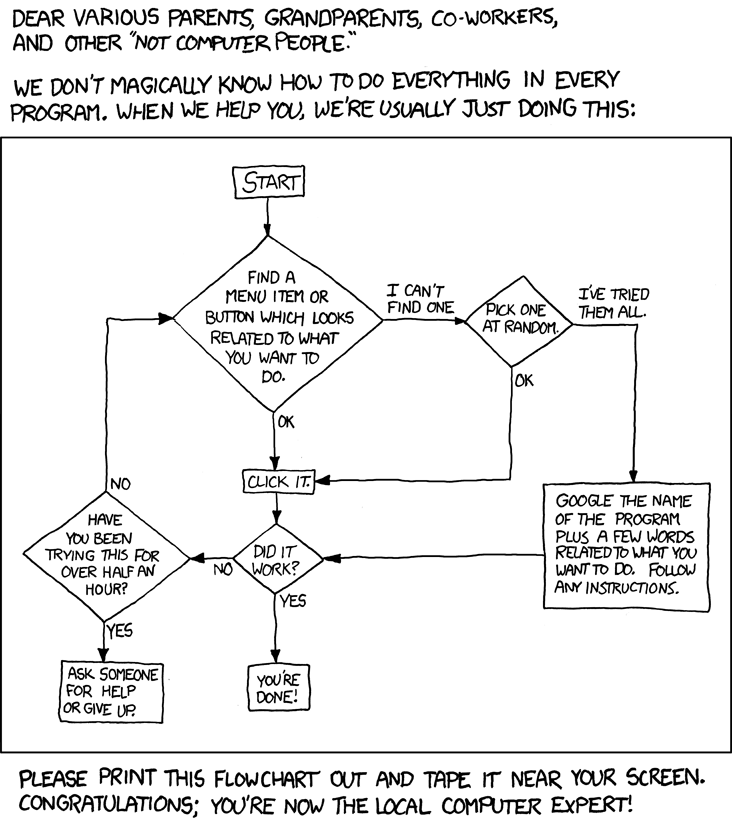
\includegraphics[height=5in]{xkcd_techsupport.png}
\end{figure}

\end{document}
